\documentclass[12pt]{exam}


\usepackage{cmap, type1ec}
\usepackage[T2A]{fontenc}
\usepackage[utf8]{inputenc}
\usepackage[russian]{babel}

\usepackage{hyperref}
\usepackage{alltt}

\usepackage[left=1cm, right=1cm, top=1.5cm, bottom=1cm]{geometry}
\usepackage{amsmath,amssymb}
\usepackage{multicol}
\usepackage{etoolbox}

\usepackage{tikz}
\usetikzlibrary{trees}
\usetikzlibrary{shapes.geometric}
\usetikzlibrary{positioning}

\newtoggle{first}
\toggletrue{first}
\togglefalse{first}

\newcommand{\class}{Теория алгоритмов}
\newcommand{\term}{Весенний семестр 2018}
\newcommand{\examnum}{Экзамен}
\newcommand{\examdate}{28 июня 2018}
\newcommand{\timelimit}{9:00 -- 12:00}

\pagestyle{head}
\firstpageheader{}{}{}
\runningheader{\class}{\examnum\ - Страница \thepage\ из \numpages}{\examdate}
\runningheadrule

\providecommand{\abs}[1]{\left\lvert{#1}\right\rvert}

\renewcommand{\solutiontitle}{}

\makeatletter
\newcommand{\iftoggleverb}[1]{%
  \ifcsdef{etb@tgl@#1}
    {\csname etb@tgl@#1\endcsname\iftrue\iffalse}
    {\etb@noglobal\etb@err@notoggle{#1}\iffalse}%
}
\makeatother

\graphicspath{{./figures/}}


\begin{document}

\noindent
\begin{tabular*}{\textwidth}{l @{\extracolsep{\fill}} r @{\extracolsep{6pt}} l}
\textbf{\class} & \textbf{Студент:} & \makebox[3in]{\hrulefill}\\
\textbf{\term} &&\\
\textbf{\examnum} &&\\
\textbf{\examdate} \\
\textbf{\timelimit}
\end{tabular*}\\
\rule[2ex]{\textwidth}{2pt}%
\begin{center}
Оценки (заполняется преверяющими)\\
\addpoints
\gradetable[h][questions]
\end{center}
\noindent
\rule[2ex]{\textwidth}{2pt}

{\bf N.B.: кроме явных оговорок, каждая задача подразумевает наличие подробного решения и/или доказательства, предшествующего ответу. В противном случае задача не будет засчитана.}

\begin{questions}


\question[7] Отметьте только {\bf верные} утверждения из списка. Обосновывать свой выбор не требуется.
\begin{checkboxes}
    \choice Алгоритм Дейкстры не завершается, если в графе есть рёбра с отрицательными весами.
        \begin{solution}
        Неверно. Алгоритм гарантированно завершается после $E$ «ослаблений» и $V+E$ операций над очередью с приоритетом. В случае с отрицательными весами он просто даст некорректный результат.
        \end{solution}

    \CorrectChoice Для ориентированного графа можно определить за время $O(V + E)$, является ли он деревом (связным графом без циклов).
        \begin{solution}
        Поиск в глубину или ширину для графа, представленного в виде списка смежных вершин, как раз занимает время $O(V+E)$.
        \end{solution}

    \choice Даны отсортированные массивы $A_1$, $A_2$ и $A_3$, каждый из которых содержит $n$ вещественных чисел. Построение сбалансированного бинарного дерева, содержащего все эти числа, займёт $\Theta(n \log n)$.
        \begin{solution}
        Массивы можно слить в один отсортированный массив за время $O(n)$. Далее, из этого массива можно построить сбалансированное дерево за $O(n)$: делаем медиану (= средний элемент) корнем дерева, левую и правую части массива отсылаем в соответствующие поддеревья. Рекурсивно проделываем то же самое для поддеревьев.
        \end{solution}

    \choice Вычисление медианы $n$-элементного массива занимает время $\Omega(n \log n)$.
        \begin{solution}
        С помощью quickselect можно найти медиану за $O(n)$
        \end{solution}

    \CorrectChoice Поиск в глубину в графе, представленном матрицей смежности, занимает время $O(V^2)$
        \begin{solution}
        В матрице смежности для любого узла поиск смежных с ним требует полного прохода по строке/столбцу. Он занимает $O(V)$, и при поиске в глубину выполяется для каждого узла. Следовательно, общее время поиска составит $O(V^2)$.
        \end{solution}

    \choice Массив {\tt [10, 3, 5, 1, 4, 2]} является max-heap
        \begin{solution}
        Представим в виде дерева:
        \begin{center}
            \begin{tikzpicture}[level distance=1cm,
              level 1/.style={sibling distance=1.5cm},
              level 2/.style={sibling distance=0.7cm}]
              \node {10}
                child {node {3}
                  child {node {1}}
                  child {node {4}}
                }
                child {node {5}
                    child {node {2}}
                    child[missing]
                };
            \end{tikzpicture}
        \end{center}
        Узел <<4>> нарушает свойство max-heap, являясь больше своего родителя. Следовательно, массив не является max-heap.
        \end{solution}

    \choice Среди упомянутых в курсе сортировок на основе сравнения, selection sort обеспечивает наименьшее время работы, когда все сортируемые элементы равны
        \begin{solution}
            Вне зависимости от значений элементов, selection sort на каждой интерации будет искать минимум на всём остатке массива. Время его работы по-прежнему составит $O(n^2)$.

            В то же время, в insertion sort добавление нового элемента в отсортированый префикс будет занимать $O(1)$: достаточно проверить, что предыдущий элемент не больше текущего. Всего совершается $n$ таких добавлений. Следовательно, время работы insertion sort на массиве одинаковых элементов составит $O(n)$.
        \end{solution}
    \end{checkboxes}


\question[3] Дана хэш-таблица, содержащая всего один ключ $k$, лежащий в одной из $m$ доступных ячеек. Используемая хэш-функция равновероятно распределяет случайные ключи по ячейкам.
Выполним в этой хэш-таблице $r$ операций поиска ключей {\em не равных} $k$. Вычислите вероятность того, что хотя бы одна из $r$ операций попадёт в ячейку, занимаемую ключом $k$.

\begin{solution}
Вероятность, что одна операция поиска {\it не попадёт} в ячейку с $k$:
$$
\frac{m-1}{m} = 1 - \frac{1}{m}
$$
Вероятность, что все $r$ операций {\it не попадут} в эту ячейку:
$$
\left(1 - \frac{1}{m}\right)^r
$$
Вероятность, что хотя бы одна операция {\it попадёт} в эту ячейку:
$$
1 - \left(1 - \frac{1}{m}\right)^r
$$


\end{solution}



\question[3] Какой алгоритм реализует анонимная функция {\tt foo}? Ответ пояснить

\begin{verbatim}
foo  = lambda l: (
    foo([i for i in l[1:] if i < l[0]])
    + [l[0]] + foo([j for j in l[1:] if j >= l[0]]) if l else []
)
\end{verbatim}

\begin{solution}
Это non-inplace Quicksort. Функция берёт первый элемент в качестве опорного, составляет два новых массива с элементами меньшими и большими опорного соответственно, и рекурсивно применяется к ним.

В отличие от in-place варианта, {\tt partition} здесь осуществляется простой конкатенацией «левого» массива, опорного элемента и «правого» массива.
\end{solution}

\question[4] Докажите или опровергните утверждение: чтобы удалить из min-heap элемент по $i$-му индексу, достаточно выполнить следующие действия:
\begin{itemize}
    \item обменять его местами с последним элементом массива;
    \item удалить последний элемент массива;
    \item вызывать {\tt min\_heapify} для $i$-го индекса чтобы восстановить корректность кучи.
\end{itemize}

\begin{solution}
{\bf N.B.:} на самом экзамене был дан другой, двусмысленный вариант этой задачи. Я слишком поздно заметил ошибку, поэтому очень лояльно проверял решения исходя из индивидуальной интерпретации задачи каждым студентом.

Под {\tt min-heapify} в задаче понимается аналог функции {\tt max-heapify} из CLRS 6.2. Она восстаналивает свойство min-heap для дерева с корнем $i$, предполагая, что деревья с корнями {\tt left(i)} и {\tt right(i)} {\it уже являются} корректными min-heaps. 

\begin{verbatim}
def min_heapify(A, i, n):
    l, r = left(i), right(i)
    smallest = i

    if l < n and A[l] < A[smallest]:
        smallest = l

    if r < n and A[r] < A[smallest]:
        smallest = r

    if smallest != i:
        A[i], A[smallest] = A[smallest], A[i]
        min_heapify(A, smallest, n)
\end{verbatim}

Теперь, рассмотрим min-heap:
\begin{center}
    \begin{tikzpicture}[level distance=0.7cm,
      level 1/.style={sibling distance=2cm},
      level 2/.style={sibling distance=1cm},
      level 3/.style={sibling distance=0.9cm},
      ]
      \node {1}
        child {node {10}
          child {node {20}
            child {node {40}}
            child {node {50}}
          }
          child {node {30}}
        }
        child {node {100}
            child {node {200}}
            child {node {300}}
        };
    \end{tikzpicture}   
\end{center}

Мы хотим удалить элемент 200. Выполняя первые два шага предложенного алгоритма, получаем:
\begin{center}
    \begin{tikzpicture}[level distance=0.7cm,
      level 1/.style={sibling distance=2cm},
      level 2/.style={sibling distance=1cm},
      level 3/.style={sibling distance=0.9cm},
      ]
      \node {1}
        child {node {10}
          child {node {20}
            child {node {40}}
            child[missing]
          }
          child {node {30}}
        }
        child {node {100}
            child {node {{\bf 50}}}
            child {node {300}}
        };
    \end{tikzpicture}   
\end{center}

Но 50 меньше своего родителя 100, что нарушает свойство min-heap. Выполнение {\tt min\_heapify} над индексом с элементом 50 не исправит этого нарушения: 50 всё равно останется в левом поддереве вершины 100. Значит, алгоритм в условии {\bf не является корректным}. 
\end{solution}



\question[5] Перечислите {\bf все} бинарные деревья, где порядок обхода узлов совпадает при обходах
\noaddpoints
\begin{parts}
    \part[3] preorder и inorder
    \part[1] preorder и postorder
    \part[1] inorder и postorder
\end{parts}
\addpoints
Считать что в бинарных деревьях нет повторяющихся элементов

\begin{solution}[\fill]
    \begin{enumerate}
        \item[(a)] Любые бинарные деревья без левых ребёр:
        \begin{center}
            \begin{tikzpicture}[level distance=1cm,
              level 1/.style={sibling distance=1.5cm},
              level 2/.style={sibling distance=1cm}]
              \node[draw,circle] {}
                child[missing]
                child {
                  node[draw,circle] {}
                  child[missing]
                  child {
                    node {$\cdots$}
                    child[missing]
                    child {node[draw,circle] {}}
                  }
                };
            \end{tikzpicture}
        \end{center}
        \item[(b)] Бинарное дерево только с одним узлом и пустое дерево.
        \item[(c)] Любые бинарные деревья без правых ребёр.
    \end{enumerate}
\end{solution}


\question[7] Дан кольцевой буфер, содержащий $n$ целых (в том числе отрицательных) чисел. Опишите эффективный алгоритм, вычисляющий максимальную сумму, составленную из смежных элементов кольцевого буфера.\footnote{Первый и последний элемент массива, представляющего кольцевой буфер, считаются смежными.} Пример: в буфере {\tt [1, 5, -10, 13, -5]} такая максимальная сумма равна $14$ $(13 + (-5) + 1 + 5)$

\begin{solution}
Используя динамическое программирование, следует вычислить все возможные суммы смежных элементов, перебирая индекс первого элемента $i$ и количество элементов $k$. Реализуемое рекуррентное соотношение выглядит так:
$$
S(i, k) = S(i, k-1) + A(i+k-1 \mod n)
$$
Всего будет вычислено $n^2$ значений за время $O(n^2)$, из которых нужно выбрать максимум.

\newpage

Оптимизированный вариант алгоритма, в котором таблица значений $S$ не хранится в явном виде, может выглядеть так:
\begin{verbatim}
def get_max_sum(seq):
    n = len(seq)
    max_sum = float('-inf')
    
    for i in range(n):
        partial = 0
        for k in range(n):
            partial += seq[(i + k) % n]
            max_sum = max(max_sum, partial)

    return max_sum
\end{verbatim}


\end{solution}


\question[8] Напишите рекурсивную функцию, возвращающую список наибольших чисел с каждого горизонтального уровня бинарного дерева. Например:


\begin{verbatim}
Input:    1           Output: [1, 3, 9]
         / \
        3   2
       / \   \  
      5   3   9 
\end{verbatim}


Считайте, что узлы дерева содержат только положительные числа. Решение должно состоять ровно из одной рекурсивной функции:

\begin{verbatim}
class Node(object):          def max_by_layers(self, root: Node) -> List[int]:
    value: int                   ...
    left: Node
    right: Node
\end{verbatim}


\begin{solution} \
Если вызвать эту функцию рекурсивно для потомков, мы получим списки наибольших значений с каждого из уровней левого и правого поддеревьев. Теперь достаточно сравнить их попарно и выбрать максимальные. Важно, что эти списки могут быть разной длины. Для их попарного сравнения подойдёт {\tt itertools.zip\_longest}. Но вместо этого можно удлиннить более короткий массив и применить стандартный {\tt zip}:
\begin{verbatim}
def max_by_layers(root):
    if not root:
        return []

    left = max_by_layers(root.left)
    right = max_by_layers(root.right)

    nl, nr = len(left), len(right)

    # Extend one of the arrays to equalise the lenght
    shorter = left if (nl < nr) else right
    shorter.extend([float('-inf')] * abs(nl - nr))

    maxes = (max(a, b) for a, b in zip(left, right))

    return [root.value, *maxes]
\end{verbatim}
\end{solution}


\question[10] Рассмотрим граф состояний некоторой игры. Веса на рёбрах обозначают вероятности того, что вы сможете перейти из одного состояния в другое. Цель игры -- перейти от состояния $s$ к состоянию $t$. Опишите такое преобразование графа, чтобы алгоритм Дейкстры смог найти в нём путь от $s$ к $t$, на котором вероятность выигрыша максимально возможная.

\begin{figure}[h!]
\begin{center}
  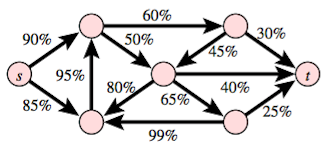
\includegraphics[width=10cm]{weighted.png}
  \end{center}
\end{figure}


\begin{solution} \
Пусть $e_1, e_2, ..., e_k$ -- список рёбер на некотором пути от $s$ до $t$. Вероятность успешно пройти этот путь равна $p(e_1) \cdot p(e_2) \cdot ... \cdot p(e_k)$, как вероятность одновременного выполнения независимых событий. Именно это произведение нам необходимо {\it максимизировать}. Алгоритм Дейкстры, однако, {\it минимизирует сумму весов} $w(e_1) + w(e_2) + w(e_2) + ... w(e_k)$. Это не то, что нам нужно.

Но если переопределить веса, прологарифмировав их с обратным знаком:
$$
w(e_i) = -\log p(e_i)
$$

то, используя свойство суммы логарифмов и учитывая отрицательный знак, минимум суммы таких весов будет приходиться на максимум произведения вероятностей:
$$
\sum w(e_i) = -\log \prod p(e_i)
$$

Обратите внимание, что $0 \leqslant p(e) \leqslant 1$, поэтому $0 \leqslant -\log p(e) < +\infty$. Новые веса неотрицательны, а значит к графу можно применять алгоритм Дейкстры.
\end{solution}




\question[3] На рисунке изображен подграф метро Санкт-Петербурга. Весом рёбер в нём является время ходьбы пешком между станциями. Пунктирные рёбра, не соответсвующие линиям метро, тоже являются частью графа. Пересадочные станции считаются одной вершиной.

Выделите на этом графе минимальное покрывающее дерево. Кратко запишите ход его построения.

\vspace{2cm}

\begin{figure}[ht!]
\begin{center}
  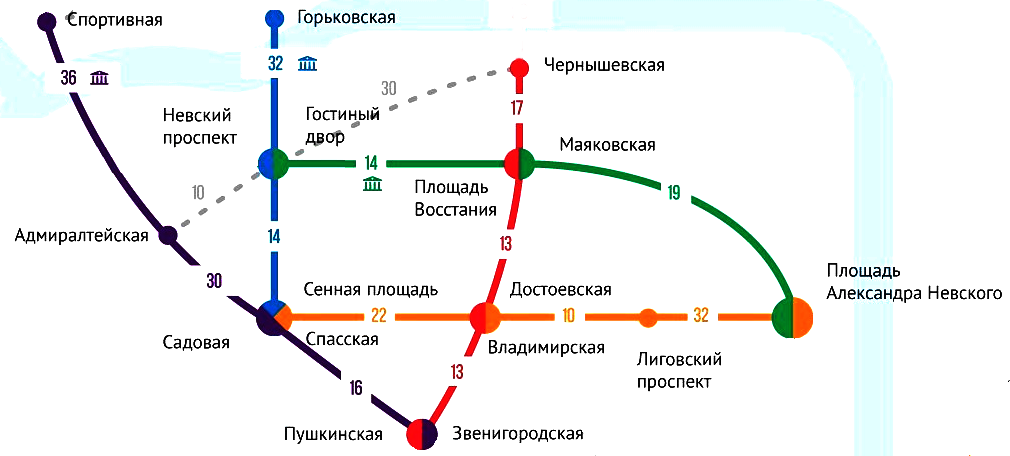
\includegraphics[width=23cm]{spb.png}
  \end{center}
\end{figure}

\begin{solution}
Воспользуемся алгоритмом Прима:
\begin{itemize}
    \item добавляем в минимальное покрывающее дерево (MST) произвольный узел: {\it Спортивная};
    \item по одному добавляем в MST минимальные рёбра (кроме тех, которые ведут к уже добавленым узлам). Получается последовательность весов: 36, 10, 14 (Гостинный-Восстания), 13, 10, 13, 17, 19, 32;
    \item все вершины покрыты, MST построено.
\end{itemize}
\end{solution}



\end{questions}

\end{document}